\documentclass[crop,tikz,margin=2pt]{standalone}% 'crop' is the default for v1.0, before it was 'preview'
%\usetikzlibrary{...}% tikz package already loaded by 'tikz' option

\usepackage{newtxmath}
\usepackage{newtxtext}



\begin{document}




\tikzset{every picture/.style={line width=0.75pt}} %set default line width to 0.75pt        

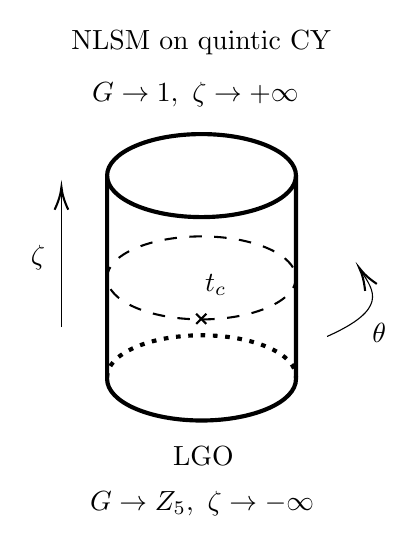
\begin{tikzpicture}[x=0.75pt,y=0.75pt,yscale=-1,xscale=1]
%uncomment if require: \path (0,300); %set diagram left start at 0, and has height of 300

%Shape: Ellipse [id:dp2741149104013215] 
\draw  [line width=1.5]  (91.5,96.5) .. controls (91.5,85.45) and (111.87,76.5) .. (137,76.5) .. controls (162.13,76.5) and (182.5,85.45) .. (182.5,96.5) .. controls (182.5,107.55) and (162.13,116.5) .. (137,116.5) .. controls (111.87,116.5) and (91.5,107.55) .. (91.5,96.5) -- cycle ;
%Shape: Arc [id:dp4483177494504115] 
\draw  [draw opacity=0][line width=1.5]  (182.45,193.56) .. controls (182.48,193.87) and (182.5,194.18) .. (182.5,194.5) .. controls (182.5,205.55) and (162.13,214.5) .. (137,214.5) .. controls (111.87,214.5) and (91.5,205.55) .. (91.5,194.5) .. controls (91.5,194.31) and (91.51,194.11) .. (91.52,193.92) -- (137,194.5) -- cycle ; \draw  [line width=1.5]  (182.45,193.56) .. controls (182.48,193.87) and (182.5,194.18) .. (182.5,194.5) .. controls (182.5,205.55) and (162.13,214.5) .. (137,214.5) .. controls (111.87,214.5) and (91.5,205.55) .. (91.5,194.5) .. controls (91.5,194.31) and (91.51,194.11) .. (91.52,193.92) ;  
%Shape: Arc [id:dp2927743480680205] 
\draw  [draw opacity=0][dash pattern={on 1.69pt off 2.76pt}][line width=1.5]  (91.52,193.92) .. controls (91.51,193.76) and (91.51,193.6) .. (91.51,193.44) .. controls (91.51,182.4) and (111.88,173.44) .. (137.01,173.44) .. controls (162.14,173.44) and (182.51,182.4) .. (182.51,193.44) -- (137.01,193.44) -- cycle ; \draw  [dash pattern={on 1.69pt off 2.76pt}][line width=1.5]  (91.52,193.92) .. controls (91.51,193.76) and (91.51,193.6) .. (91.51,193.44) .. controls (91.51,182.4) and (111.88,173.44) .. (137.01,173.44) .. controls (162.14,173.44) and (182.51,182.4) .. (182.51,193.44) ;  
%Straight Lines [id:da5072276241930813] 
\draw [line width=1.5]    (91.5,96.5) -- (91.52,193.92) ;
%Straight Lines [id:da6889614182434406] 
\draw [line width=1.5]    (182.5,96.5) -- (182.52,193.92) ;
%Shape: Arc [id:dp03737706744165514] 
\draw  [draw opacity=0][dash pattern={on 4.5pt off 4.5pt}][line width=0.75]  (182.44,144.85) .. controls (182.47,145.16) and (182.49,145.47) .. (182.49,145.79) .. controls (182.49,156.84) and (162.12,165.79) .. (136.99,165.79) .. controls (111.86,165.79) and (91.49,156.84) .. (91.49,145.79) .. controls (91.49,145.17) and (91.56,144.55) .. (91.68,143.95) -- (136.99,145.79) -- cycle ; \draw  [dash pattern={on 4.5pt off 4.5pt}][line width=0.75]  (182.44,144.85) .. controls (182.47,145.16) and (182.49,145.47) .. (182.49,145.79) .. controls (182.49,156.84) and (162.12,165.79) .. (136.99,165.79) .. controls (111.86,165.79) and (91.49,156.84) .. (91.49,145.79) .. controls (91.49,145.17) and (91.56,144.55) .. (91.68,143.95) ;  
%Shape: Arc [id:dp2626843324028918] 
\draw  [draw opacity=0][dash pattern={on 4.5pt off 4.5pt}][line width=0.75]  (91.5,146.27) .. controls (91.49,146.11) and (91.49,145.95) .. (91.49,145.79) .. controls (91.49,134.74) and (111.86,125.79) .. (136.99,125.79) .. controls (162.12,125.79) and (182.49,134.74) .. (182.49,145.79) -- (136.99,145.79) -- cycle ; \draw  [dash pattern={on 4.5pt off 4.5pt}][line width=0.75]  (91.5,146.27) .. controls (91.49,146.11) and (91.49,145.95) .. (91.49,145.79) .. controls (91.49,134.74) and (111.86,125.79) .. (136.99,125.79) .. controls (162.12,125.79) and (182.49,134.74) .. (182.49,145.79) ;  
\draw  [line width=0.75]  (134.43,163.07) -- (139.28,167.93)(139.28,163.07) -- (134.43,167.93) ;
%Curve Lines [id:da03517070430844493] 
\draw    (197.5,174) .. controls (227.27,160.77) and (219.97,152.01) .. (214.02,142.64) ;
\draw [shift={(213,141)}, rotate = 59.04] [color={rgb, 255:red, 0; green, 0; blue, 0 }  ][line width=0.75]    (10.93,-3.29) .. controls (6.95,-1.4) and (3.31,-0.3) .. (0,0) .. controls (3.31,0.3) and (6.95,1.4) .. (10.93,3.29)   ;
%Straight Lines [id:da06223204606509136] 
\draw    (69.5,169.5) -- (69.5,104) ;
\draw [shift={(69.5,102)}, rotate = 90] [color={rgb, 255:red, 0; green, 0; blue, 0 }  ][line width=0.75]    (10.93,-3.29) .. controls (6.95,-1.4) and (3.31,-0.3) .. (0,0) .. controls (3.31,0.3) and (6.95,1.4) .. (10.93,3.29)   ;

% Text Node
\draw (137.5,142.9) node [anchor=north west][inner sep=0.75pt]    {$t_{c}$};
% Text Node
\draw (218,166.4) node [anchor=north west][inner sep=0.75pt]    {$\theta $};
% Text Node
\draw (53.5,128.9) node [anchor=north west][inner sep=0.75pt]    {$\zeta $};
% Text Node
\draw (122,226) node [anchor=north west][inner sep=0.75pt]   [align=left] {LGO};
% Text Node
\draw (73,25.5) node [anchor=north west][inner sep=0.75pt]   [align=left] {NLSM on quintic CY};
% Text Node
\draw (82,247.4) node [anchor=north west][inner sep=0.75pt]    {$G\rightarrow \vvmathbb{Z}_{5} ,\ \zeta \rightarrow -\infty $};
% Text Node
\draw (83,50.4) node [anchor=north west][inner sep=0.75pt]    {$G\rightarrow 1,\ \zeta \rightarrow +\infty $};


\end{tikzpicture}
\end{document}